
\subsection{BÀI TẬP TRẮC NGHIỆM}

\Opensolutionfile{ans}[ans/1H4.B5]
\setcounter{ex}{0}
\begin{ex}
	Cho hình hộp $ABCD.A'B'C'D'$  . Gọi $M, M'$   lần lượt là trung điểm của các cạnh $BC, B'C'$  Hình chiếu của $\Delta B'DM$  qua phép chiếu song song trên $(A'B'C'D')$  theo phương chiếu $AA'$   là
	\choice
	{$\Delta B'A'M'$}
		{$\Delta C'D'M'$}
			{$\Delta DMM'$}
				{\True$\Delta B'D'M'$}
\end{ex}
\begin{ex}
		Cho hình hộp $ABCD.A'B'C'D'$  . Gọi $M, M'$   lần lượt là trung điểm của các cạnh $BC, B'C'$  Hình chiếu của $\Delta D'CM$  qua phép chiếu song song trên $(A'B'C'D')$  theo phương chiếu $BB'$   là
	\choice
	{$\Delta B'CM'$}
	{\True$\Delta C'D'M'$}
	{$\Delta DMM'$}
	{$\Delta B'D'M'$}
\end{ex}
\begin{ex}
	Cho hình hộp $ABCD.A'B'C'D'$  . Gọi $M, M'$   lần lượt là trung điểm của các cạnh $AD, A'D'$; $N, N'$ lần lườ là trung điểm của các cạnh $CD, C'D'$; $P$ là trung điểm của $DD'$.  Hình chiếu của $\Delta MNP$  qua phép chiếu song song trên $(A'B'C'D')$  theo phương chiếu $BB'$   là
	\choice
	{$\Delta B'N'M'$}
	{\True$\Delta D'M'N'$}
	{$\Delta PM'N'$}
	{$\Delta PD'M'$}
\end{ex}
\begin{ex}
	Trong các mệnh đề sau, có bao nhiêu mệnh đề đúng?
	\begin{itemize}
		\item [a)] Một đường thẳng có thể song song với hình chiếu của nó.
		\item [b)] Một đường thẳng có thể trùng với hình chiếu của nó.
		\item [c)] Hình chiếu song song của hai đường thẳng chéo nhau có thể song song với nhau.
		\item [d)]Hình chiếu song song của hai đường thẳng chéo nhau có thể trung nhau.
	\end{itemize}
\choice
{$1$}
{$2$}
{$3$}
{$4$}
\end{ex}
\begin{ex}
	Trong các mệnh đề sau, có bao nhiêu mệnh đề đúng?
	\begin{itemize}
		\item [a)] Phép chiếu song song biến đoạn thẳng thành đoạn thẳng.
		\item [b)] Phép chiếu song song biến hai đường thẳng song song thành hai đường thẳng cắt nhau.
		\item [c)] Phép chiếu song song biến tam giác đều thành tam giác cân.
		\item [d)] Phép chiếu song song biến hình vuông thành hình bình hành.
	\end{itemize}
	\choice
	{$1$}
	{$2$}
	{$3$}
	{$4$}
\end{ex}

\begin{ex}%[1H2K5]
	Hình chiếu của tứ diện $ABCD$ lên một mặt phẳng $(P)$ theo phương chiếu $AB$ ($AB$ không song song với $(P)$ là
	\choice{\True hình tam giác}
	{hình tứ giác}
	{đoạn thẳng}
	{hình thang}
\end{ex}

\begin{ex}%[1H2K5]
	Hình nào dưới đây \textbf{không phải} là hình biểu diễn của một tứ diện?
	\def\dotEX{}
	\choice{
		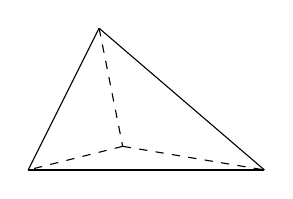
\begin{tikzpicture}[scale=0.3]
			\draw (3.,6.)-- (0.,0.);
			\draw (0.,0.)-- (10.,0.);
			\draw (3.,6.)-- (10.,0.);
			\draw [dashed](3.,6.)-- (4.,1.);
			\draw [dashed](4.,1.)-- (0.,0.);
			\draw [dashed](4.,1.)-- (10.,0.);
		\end{tikzpicture}	
	}{
		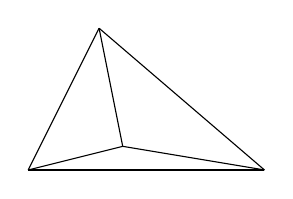
\begin{tikzpicture}[scale=0.3]
			\draw (3.,6.)-- (0.,0.);
			\draw (0.,0.)-- (10.,0.);
			\draw (3.,6.)-- (10.,0.);
			\draw (3.,6.)-- (4.,1.);
			\draw (4.,1.)-- (0.,0.);
			\draw (4.,1.)-- (10.,0.);
		\end{tikzpicture}	
	}{
		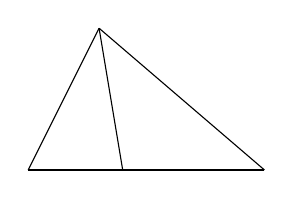
\begin{tikzpicture}[scale=0.3]
			\draw (3.,6.)-- (0.,0.);
			\draw (0.,0.)-- (10.,0.);
			\draw (3.,6.)-- (10.,0.);
			\draw (3.,6.)-- (4.,0.);
		\end{tikzpicture}	
	}{
		\True
		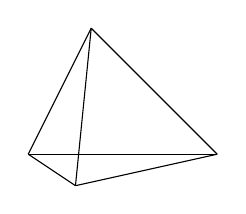
\begin{tikzpicture}[scale=0.2]
			\draw (4.,8.)-- (0.,0.);
			\draw (4.,8.)-- (12.,0.);
			\draw (0.,0.)-- (3.,-2.);
			\draw (3.,-2.)-- (12.,0.);
			\draw (4.,8.)-- (3.,-2.);
			\draw (0.,0.)-- (12.,0.);
		\end{tikzpicture}	
	}
\end{ex}



\begin{ex}%[Võ Đông Phước]%[1D1G2]
	Cho hình lăng trụ tam giác $ABC.A'B'C'$. Gọi $M, M'$ lần lượt là trung điểm của các cạnh $BC, B'C'$ và $I$ là giao điểm của đường thẳng $A'M$ và $(AB'C')$. Tìm hình chiếu song song của $I$ trên $(A'B'C')$ theo phương $BB'$.
	\choice{\True Trung điểm của đoạn thẳng $A'M'$}
	{Trọng tâm của tam giác $A'B'C'$}
	{Điểm $A'$}
	{Điểm $M'$}
\end{ex}
%%%%%%%%%%%%%%%%%%%%%%%%%%%%%%%%%%%%%%%%
\begin{ex}%[Võ Đông Phước]%[1D1G2]
	Cho tứ diện $ABCD$. Gọi $M, N$ lần lượt là trung điểm của các cạnh $AC, BC$, trên cạnh $BD$ lấy điểm $P$ sao cho $BP=2PD$. Mặt phẳng $(MNP)$ cắt mặt phẳng $(ACD)$ theo giao tuyến $d$. Tìm hình chiếu song song của đường thẳng $d$ trên $(BCD)$ theo phương $AD$.
	\choice{Đường thẳng $DN$}
	{\True Đường thẳng $CD$}
	{Đường thẳng $BD$}
	{Điểm $M$}
\end{ex}

\begin{ex}%[1H2G5]
	Cho tứ diện $ABCD$ và $M$ là điểm bất kì thuộc miền trong của tam giác $BCD$. Gọi $B'$, $C'$, $D'$ lần lượt là hình chiếu song song của $M$ theo các phương $AB$, $AC$, $AD$ lên các mặt $(ACD)$, $(ABD)$, $(ABC)$. Tính $\dfrac{MB'}{AB}+\dfrac{MC'}{AC}+\dfrac{MD'}{AD}$.
	\choice{\True $1$}
	{$\dfrac{1}{9}$}
	{$\dfrac{1}{3}$}
	{$3$}
	\loigiai{
		\immini{
			Trong tam giác $ABI$ ta có $\dfrac{MB'}{AB}=\dfrac{MI}{BI}$.\\
			Tương tự ta cũng có $\dfrac{MC'}{AC}=\dfrac{MJ}{CJ}$ và $\dfrac{MD'}{AD}=\dfrac{MK}{DK}$.\\
			Dễ thấy rằng $\dfrac{S_{MBD}}{S_{CBD}}=\dfrac{MJ}{CJ}$, $\dfrac{S_{MCD}}{S_{BCD}}=\dfrac{MI}{BI}$, $\dfrac{S_{MBC}}{S_{DBC}}=\dfrac{MK}{DK}$.\\
			Cộng các đẳng thức với nhau vế theo vế ta được $$\dfrac{MB'}{AB}+\dfrac{MC'}{AC}+\dfrac{MD'}{AD}=1$$
		}{
			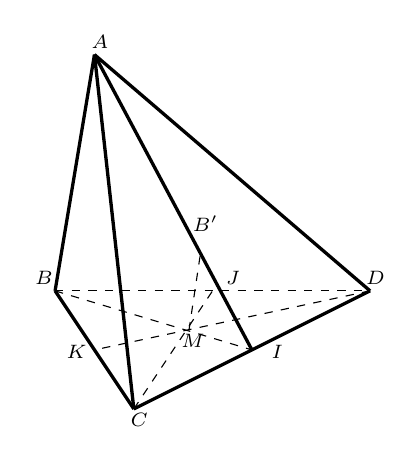
\begin{tikzpicture}[scale=0.5]
				\draw [dashed] (2.,5.)-- (10.,5.);
				\draw [line width=1.2pt] (2.,5.)-- (4.,2.);
				\draw [line width=1.2pt] (4.,2.)-- (10.,5.);
				\draw [line width=1.2pt] (3.,11.)-- (2.,5.);
				\draw [line width=1.2pt] (3.,11.)-- (4.,2.);
				\draw [line width=1.2pt] (3.,11.)-- (10.,5.);
				\draw [line width=1.2pt] (3.,11.)-- (7.,3.5);
				\draw [dashed] (2.,5.)-- (7,3.5);
				\draw [dashed] (10.,5.)-- (3.,3.5);
				\draw [dashed] (4.,2.)-- (6.,5.);
				\draw [dashed] (5.4,4)-- (5.7,6);
				\begin{scriptsize}
					\draw (2.14,5.33) node[left] {$B$};
					\draw (10.14,5.33) node {$D$};
					\draw (4.14,2.1) node [below]{$C$};
					\draw (3.14,11.33) node {$A$};
					\draw (7.3,3.83) node [below right]{$I$};
					\draw (3,3.81) node [below left]{$K$};
					\draw (6.14,5.33) node [right]{$J$};
					\draw (5.5,4.1) node [below]{$M$};
					\draw (5.82,6.31) node [above]{$B'$};
				\end{scriptsize}
			\end{tikzpicture}
		}
		
	}	
	
\end{ex}
\centerline{---HẾT---}
\Closesolutionfile{ans}